

\par Variables used for the $\nu_e$ selections aim to isolate features in the neutrino interaction that are specific to events with final-state electrons. These features are split in several categories which leverage calorimetric and topological information that characterizes $\nu_e$ interactions. This section describes the variables used in the $\nu_e$ selections. Table ~\ref{tab:variableSummary} summarizes all variables used, with a brief description. Variables that warrant a longer introduction are described below.





\begin{figure}[H]
\begin{center}
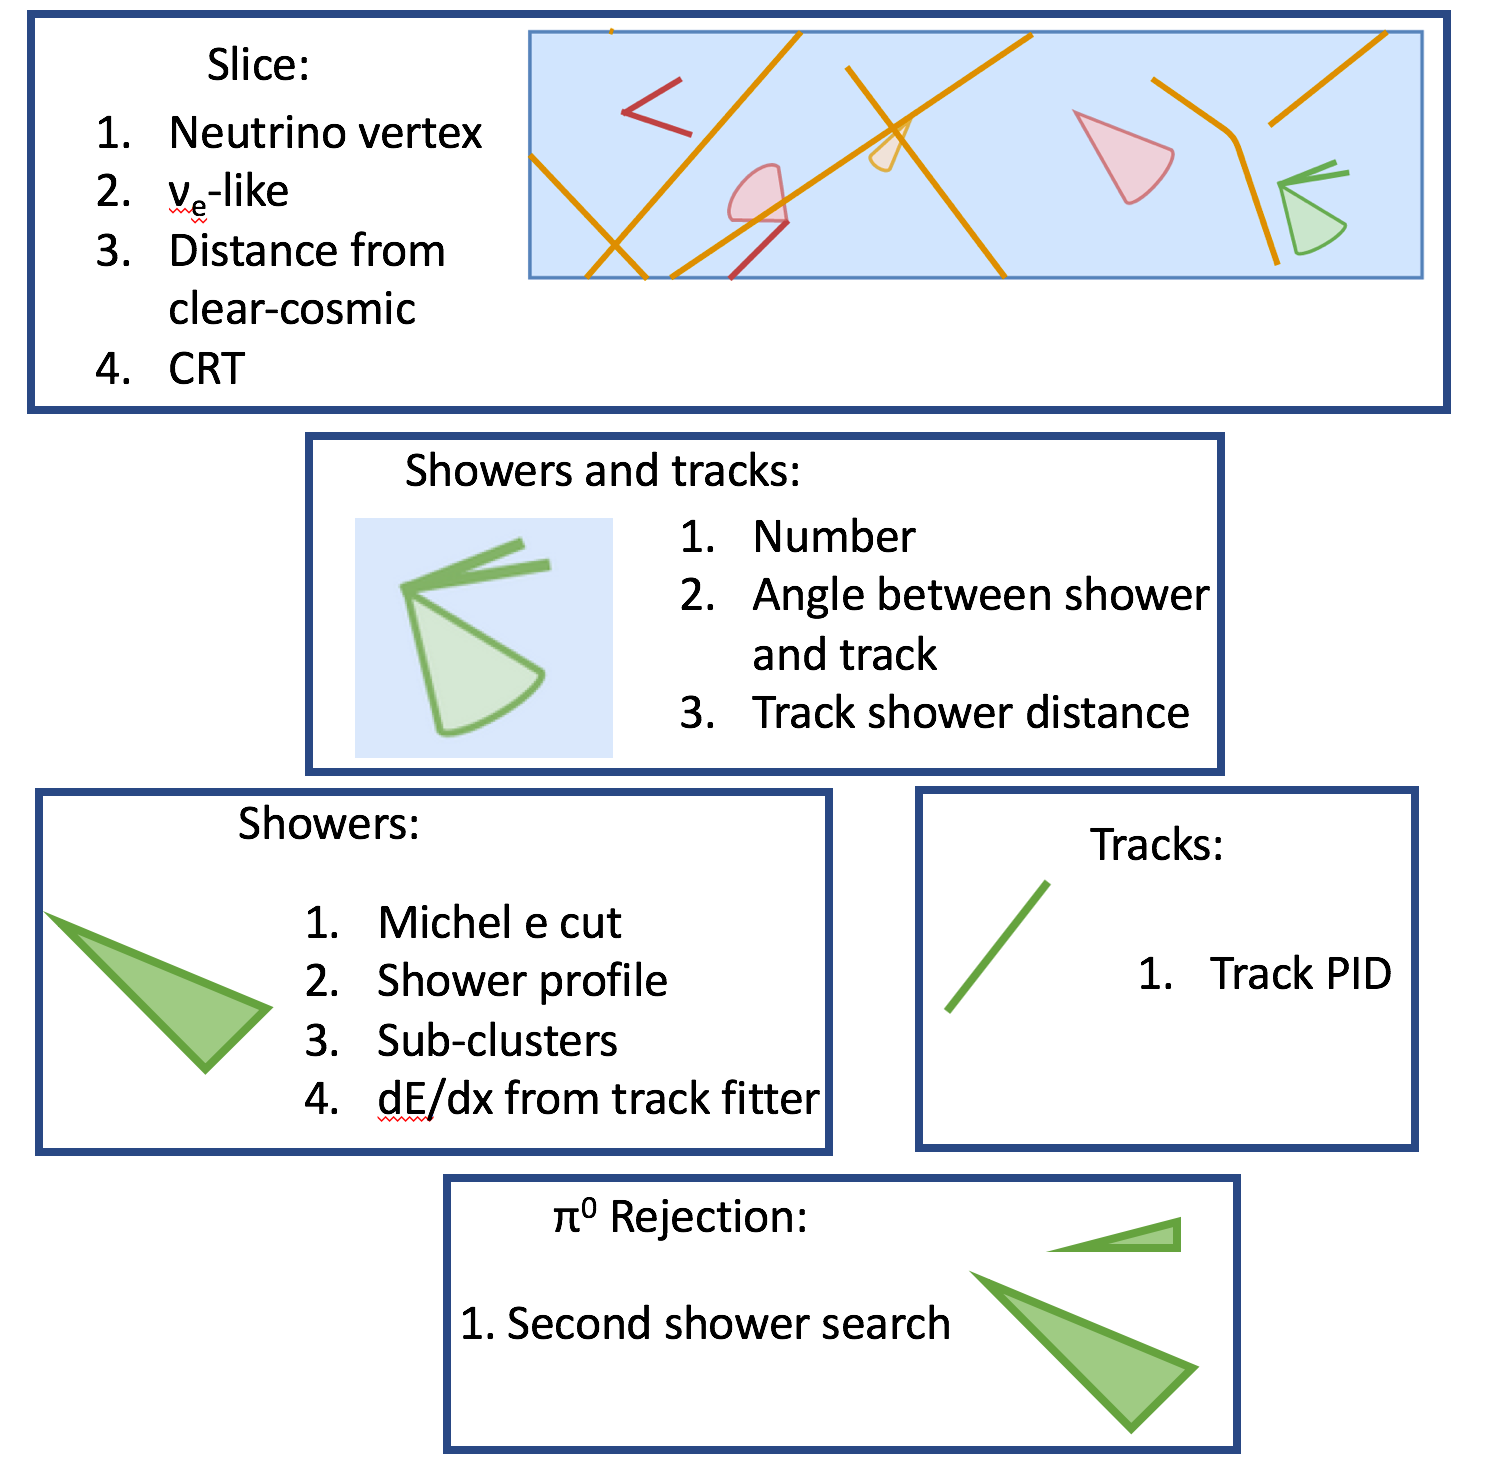
\includegraphics[width=0.6\textwidth]{nueselection/tools.png}
\caption{\label{fig:nue:variables}Categories of variables leveraged in the $\nu_e$ selections.}
\end{center}
\end{figure}

\par \noindent \textbf{track-shower separation} The first step in track-shower separation relies on the topological score reconstructed by Pandora, which utilizes inputs such as the PCA component of 3D space-points to classify PFParticles. Nonetheless, this classification is not sufficient to obtain the track-shower separation needed. To improve on this, additional variables which leverage different aspects of shower topologies are devised:

\begin{itemize}
    \item \textbf{shower track-fitted fraction} (variable: \emph{trkit}, figure~\ref{fig:nue:variables:trkfit}) This quantity is the fraction of the 3D spacepoints in a shower object that are successfully fit with the shower track-fitter algorithm. Tracks, comprised of a single contiguous segment, will be entirely fit, leading to a fraction of 1. Showers, with several branches and split charge deposition segments, will have a fraction that is less then one.
    \item \textbf{shower sub-clusters} (variable: \emph{subcluster}, figure~\ref{fig:nue:variables:subcluster}) This quantity leverages the fact that EM showers are often comprised of several branches isolated by gaps caused by photons propagating through the detector medium. The variable is calculated by counting the number of isolated 2D segments of charge associated to reconstructed showers. This quantity is a sum of such clusters from all three planes.
    \item \textbf{Moliere ``angle''} (variable: \emph{shrmoliereavg}, figure~\ref{fig:nue:variables:dedx}) This quantity aims to characterize the profile of reconstructed EM showers. It is computed using 3D spacepoints. For each 3D spacepoint, the angle between the shower's direction and the spacepoint is calculated. The average of all such angles is used as the variable.
    \item \textbf{dE/dx variables} (variable: \emph{shr\_tkfit\_gap10\_dedx\_\{U,V,Y\}} and \emph{shr\_tkfit\_2cm\_dedx\_\{U,V,Y\}} )  These variables computed using calorimetric information from each plane. The two different variables are calculated as the median d$E$/d$x$ computed over some segment of a shower's trunk. The two segments used are the first two centimeters, and the range [1,5] cm. The choice to leverage both these variables  is motivated by: (a) Sometimes - especially for the 1$e$0$p$ channel - the first few hits of a shower merge activity from short protons, causing a large d$E$/d$x$ which hampes the ability to identify the event as an electron. (b) For photon showers, especially at low energy, d$E$/d$x$ becomes more and more MIP-like as one moves further along the shower (see figure~\ref{fig:dedxgammas:dist}).
\end{itemize}{}



\begin{figure}[H] 
\begin{center}
    \begin{subfigure}[b]{0.3\textwidth}
    \centering
    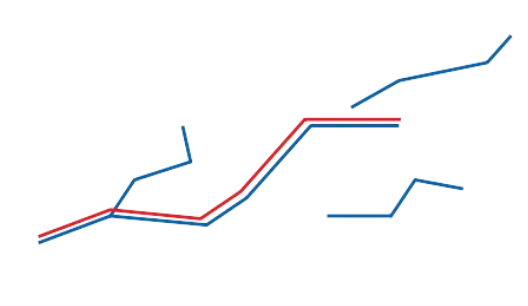
\includegraphics[width=1.00\textwidth]{nueselection/variables/trkfit.png}
    \caption{\label{fig:nue:variables:trkfit} ``trkfit'' variable }
    \end{subfigure}
    \begin{subfigure}[b]{0.3\textwidth}
    \centering
    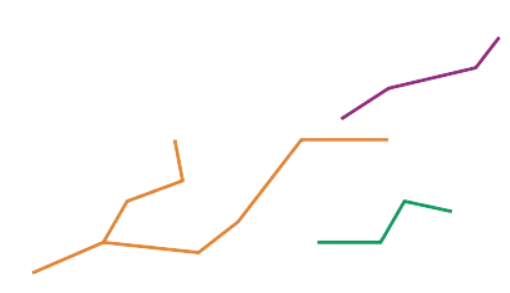
\includegraphics[width=1.00\textwidth]{nueselection/variables/nbranch.png}
    \caption{\label{fig:nue:variables:subcluster} ``subcluster'' variable }
    \end{subfigure}
    \begin{subfigure}[b]{0.3\textwidth}
    \centering
    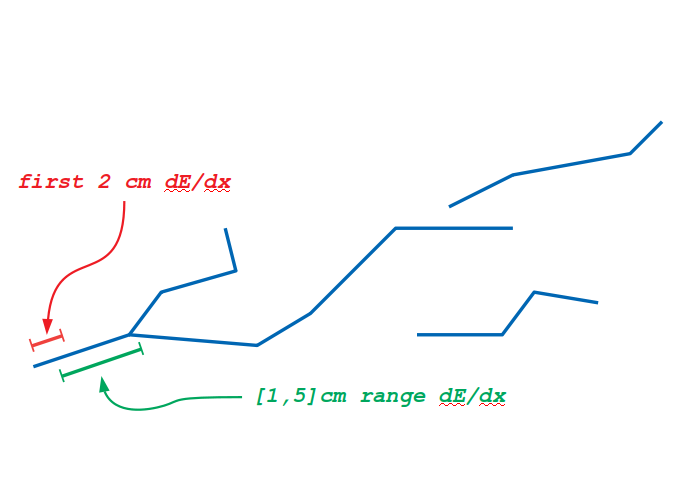
\includegraphics[width=1.00\textwidth]{nueselection/variables/dedx.png}
    \caption{\label{fig:nue:variables:dedx} d$E$/d$x$ variables }
    \end{subfigure}
\caption{\label{fig:nue:presel:eff} Additional shower variables defined by the analysis to improve track-shower separation.}
\end{center}
\end{figure}


\par \noindent \textbf{second-shower variables} Often in $\pi^0$ events one of the two EM $\gamma$ showers is not fully reconstructed by Pandora. In many cases, these second $\gamma$ showers are correctly identified by Pandora as belonging to the neutrino slice (reconstructed in 2D), but never fully reconstructed in 3D (see fig.~\ref{fig:nue:variables:secondshowerevd}). To improve on our $\pi^0$ rejection, we exploit this 2D-only information to reconstruct several variables which store information associated to the largest 2D cluster belonging to the slice on each plane. At the moment, only collection-plane variables are used. The variables, shown graphically in figure~\ref{fig:nue:variables:secondshower}, are described below. In the example event of figure~\ref{fig:nue:variables:secondshowerevd} these quantities are computed for the circles black cluster of charge.
\begin{itemize}
    \item \emph{secondshower\_Y\_nhit}: number of hits in the collection plane of the largest cluster associated to the  recovered 2nd shower
    \item \emph{secondshower\_Y\_dot}: dot product between the vector connecting the vertex to the closest hit in cluster and the charge-weighted cluster direction w.r.t. closest hit in cluster
    \item \emph{anglediff\_Y}: 2D angle difference in the collection plane between the 2nd shower and the 1st shower cluster  (cluster direction defined as charge-weighted direction of cluster w.r.t. vertex)
    \item \emph{secondshower\_Y\_vtxdist}: 2D distance from vertex for the largest 2D cluster associated to the  recovered 2nd shower in the collection plane
\end{itemize}{}




\begin{figure}[H] 
\begin{center}
    \begin{subfigure}[b]{0.35\textwidth}
    \centering
    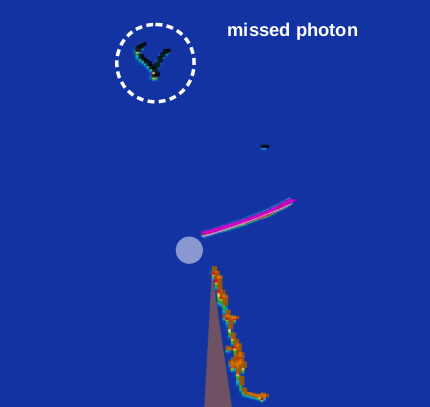
\includegraphics[width=1.00\textwidth]{nueselection/variables/secondshowerevd.png}
    \caption{\label{fig:nue:variables:secondshowerevd} ``trkfit'' variable }
    \end{subfigure}
    \begin{subfigure}[b]{0.35\textwidth}
    \centering
    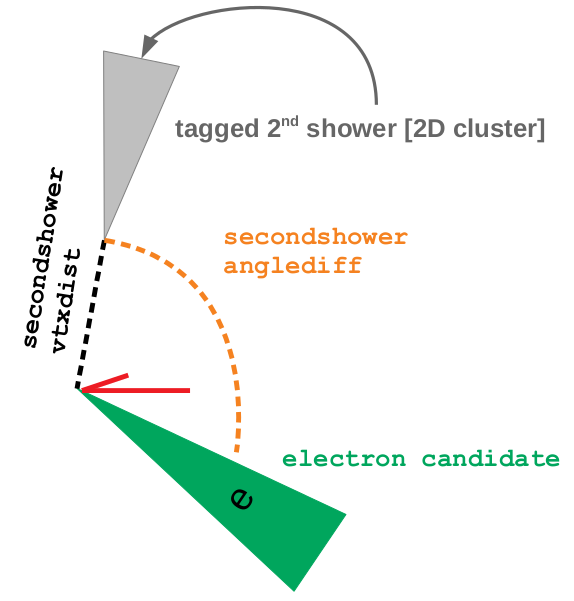
\includegraphics[width=1.00\textwidth]{nueselection/variables/secondshower.png}
    \caption{\label{fig:nue:variables:secondshower} ``subcluster'' variable }
    \end{subfigure}
\caption{\label{fig:nue:variables:secondshower} variables}
\end{center}
\end{figure}

\par \noindent \textbf{track-shower separation} In the 1$e$N$p$ channel, a gap between the shower candidate and vertex activity is a powerful $\pi^0$ rejection discriminant. We primarily rely on the measured 3D distance between the shower start point and the reconstructed start point of the longest track in the slice (variable: \emph{tksh\_distance}). Due to mis-reconstruction in the 3D shower and track reconstruction, sometimes the 3D distance just defined is reconstructed to be large (up to several centimeters) even if the individual track and shower are correctly clustered. This factors smears the track-shower separation of $\nu_e$ interactions therefore reducing the $e-\gamma$ separation power achievable. To overcome this failure specific to the 3D reconstruction, a new quantity is calculated with 2D information from the collection plane defined as the smallest 2D distance between any hits associated with the shower candidate and any hits associated with the proton candidate.


\par \noindent  \textbf{Slice variables}: these are variables associated to general features of the reconstructed neutrino interaction or event.

\begin{itemize}
    \item \emph{nslice}: Number of neutrino slices identified by the \emph{SliceID}. Values are either 0 or 1.
    \item \emph{reco\_nu\_vtx\_sce\_\{x,y,z\}}: Reconstructed space charged corrected neutrino interaction vertex in (x,y,z) coordinates.
    \item \emph{n\_showers\_contained}: number of showers with a starting point within the fiducial volume;
    \item \emph{n\_tracks\_contained}: number of tracks fully contained in the fiducial volume;
    \item \emph{contained\_fraction}: fraction of hits in PFParticles contained in the fiducial volume (according to definitions above) with respect to the total number of clustered hits in the slice;
    \item \emph{hits\_ratio}: ratio between hits from showers and total number of hits;
    \item \emph{CosmicIP}: closest distance between shower start and space points associated to tracks flagged as cosmics.
    \item \emph{crtveto}: boolean variable checking whether the event passes the CRT veto or not
    \item \emph{\_closestNuCosmicDist}: minimum 3D distance of the reconstructed neutrino vertex from a CRT-tagged cosmic track
    \item \emph{slclustfrac}: fraction of hits in the slice that are fully reconstructed to 3D particles.
\end{itemize}

\par \noindent \textbf{Shower and Track variables}:

\begin{itemize}
    \item \emph{tksh\_distance}: distance between leading shower vertex and longest track vertex;
    \item \emph{tksh\_angle}: angle between leading shower vertex and longest track vertex;
    item \emph{merge\_bestdist}: Distance between shower start point and track start (or end) point for the track in the slice that best matches the direction of the shower. 
\end{itemize}

\par \noindent \textbf{Shower variables}:

\begin{itemize}
    \item \emph{shr\_energy\_tot\_cali}: sum of the energy of the calibrated showers (in GeV). This variable is used only at pre-selection as a ``Michel veto'';
    \item \emph{shr\_tkfit\_2cm\_dedx\_\{U,V,Y\}}: dE/dx in the first 2 cm of the leading shower on plane (U,V,Y) with the track fitting;
    \item \emph{shr\_tkfit\_gap10\_dedx\_\{U,V,Y\}}: dE/dx in the [1,5] cm range of the leading shower on plane (U,V,Y) with the track fitting;
    \item \emph{shr\_score}: Pandora SVM track/shower score for the leading shower;
    \item \emph{shrmoliereavg}: average angle between the vector connecting the shower start to each shower space point and the shower direction vector
    \item \emph{subcluster}: number of subclusters (counted in all planes) for the leading shower.
    \item \emph{trkfit}: ratio of hits fitted in the track fit to the shower to all hits in the shower.
\end{itemize}

\par \noindent  \textbf{Track variables}:

\begin{itemize}
    \item \emph{trkpid}: proton-muon LLR particle identification 
\end{itemize}

\par \noindent  \textbf{2nd shower-based $\pi^0$ rejection variables}:

\begin{itemize}
    \item \emph{secondshower\_Y\_nhit}: number of hits in the collection plane of the largest cluster associated to the  recovered 2nd shower
    \item \emph{secondshower\_Y\_dot}: dot product between the vector connecting the vertex to the closest hit in cluster and the charge-weighted cluster direction w.r.t. closest hit in cluster
    \item \emph{anglediff\_Y}: 2D angle difference in the collection plane between the 2nd shower and the 1st shower cluster  (cluster direction defined as charge-weighted direction of cluster w.r.t. vertex)
    \item \emph{secondshower\_Y\_vtxdist}: 2D distance from vertex for the largest 2D cluster associated to the  recovered 2nd shower in the collection plane
\end{itemize}
